\documentclass[german, % Standardmäßig deutsche Eigenarten, englisch -> english
parskip=full, % Absätze durch Leerzeile trennen
bibliography=totoc, % Literatur im Inhaltsverzeichnis
%draft, % TODO: Entwurfsmodus -> entfernen für endgültige Version
]{scrartcl}
\usepackage{ifluatex} % zum Testen, ob LuaTeX verwendet wird
\ifluatex
\usepackage{fontspec} % Laden von Schriften
\setmainfont[Mapping=tex-text]{Linux Libertine O}  % Mapping ermöglicht die Verwendung z.B. von --
\setsansfont[Mapping=tex-text]{Linux Biolinum O}
\usepackage{polyglossia}  % Sprachpaket
\setdefaultlanguage[spelling=new,babelshorthands=true]{german}  % Neue Rechtschreibung und Abkürzungen
\else % kein LuaTeX
\usepackage[utf8]{inputenc} % Kodierung der Datei
\usepackage[T1]{fontenc} % Vollen Umfang der Schriftzeichen
\usepackage{lmodern}
\usepackage[ngerman]{babel} % Sprache auf Deutsch (neue Rechtschreibung)
%\usepackage{libertine} % Schriftart Linux Libertine/Biolinum verwenden
\fi

% Mathematik und Größen
\usepackage{amsmath}
\ifluatex
\usepackage{unicode-math}
\fi
\usepackage[locale=DE, % deutsche Eigenarten, englisch -> US
separate-uncertainty, % Unsicherheiten seperat
]{siunitx}
\usepackage{physics} % Erstellung von Gleichungen vereinfachen

% Bilder einbinden
\usepackage{graphicx}
\usepackage{float}
\usepackage{caption}
%\graphicspath{{bilder/}} % TODO: Pfad unter dem die Bilder gesucht werden

% Gestaltung
\usepackage{microtype}  % Mikrotypographie
\usepackage{booktabs}  %schönere Tabellen
\usepackage{multirow}
\usepackage[toc]{multitoc}  %mehrspaltiges Inhaltsverzeichnis
\usepackage{csquotes} % Anführungszeichen mit \enquote
\usepackage{subcaption}  % Unterabbildungen a,b,c,…
\usepackage{enumitem}  % Listen anpassen
\setlist{itemsep=-10pt}
\usepackage{scrpage2}  % Manipulation des Seitenstils
% Kopf-/Fußzeilen
\pagestyle{scrheadings}
\clearscrheadings
\automark{section}
\ofoot{\pagemark}
\ihead{\headmark}
\setheadsepline{.5pt}

\usepackage[colorlinks=true]{hyperref}  % Links und weitere PDF-Features

\makeatletter 
\renewcommand\subsection{\@startsection 
   {subsection}{2}{0mm}%      % name, ebene, einzug 
   {0.5\baselineskip}%            % vor-abstand 
   {0.3\baselineskip}%            % nach-abstand 
   {\bfseries\sffamily\large}%           % layout 
   } 
\makeatother 

% TODO: Titel und Autor, … festlegen
\newcommand*{\titel}{Optische Kohärenztomographie}
\newcommand*{\autor}{Maximilian Obst, Thomas Adlmaier}
\newcommand*{\abk}{OCT}
\newcommand*{\betreuer}{M.Sc. Jonas Golde}
\newcommand*{\messung}{28.10.2016}
\newcommand*{\ort}{Medizinische Fakultät Carl Gustav Carus}

\hypersetup{pdfauthor={\autor}, pdftitle={\titel}} % PDF-Metadaten

\titlehead{F-Praktikum \abk \hfill TU Dresden}
\subject{Versuchsprotokoll}
\title{\titel}
\author{\autor}
\date{\begin{tabular}{ll}
Protokoll: & \today\\
Messung: & \messung\\
Ort: & \ort\\
Betreuer: & \betreuer\end{tabular}}

%----------------
\begin{document}
\begin{titlepage}
\maketitle

\begin{figure}[hb] 
  \centering
     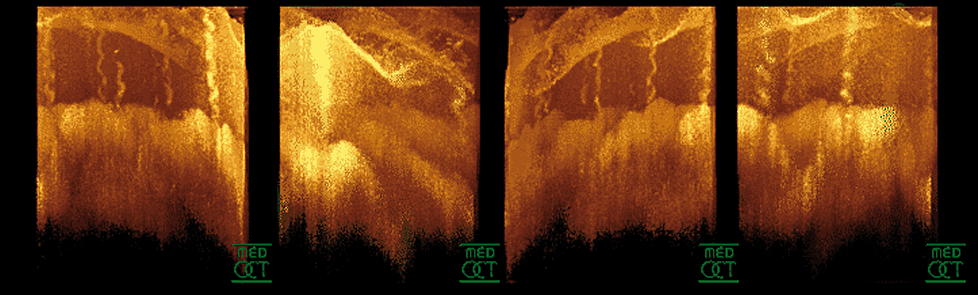
\includegraphics[width=0.7\textwidth]{tomographie}
  \caption{Fingerkuppe unter optische Kohärenztomographie	\cite{bild-tomographie}}
  \label{fig:tomographie}
\end{figure}
\end{titlepage}

\tableofcontents
\pagebreak

%------------------------
\section{Physikalische Grundlagen}

Die Optische Kohärenztomographie ist ein bildgebendes Verfahren, welches vor allem in der Humanmedizin verwendet wird. Dort schließt es die Lücke zwischen Sonographie, welche sehr tief in den Körper eindringen kann, aber nur eine grobe Auflösung bietet, und Mikrokopie, die nur die Oberfläche abbilden kann. Die optische Kohärenztomographie (OCT) bildet die ersten Millimeter des Gewebes mit hoher Auflösung ab.
In diesem Versuch wird eine Einführung in die Arbeit mit OCT geboten. Es wird sowohl Time Domain OCT als auch Frequency Domain OCT durchgeführt.

\subsection{Einführung}

Bei der OCT wird ein Material mit Licht einer bestimmten Wellenlänge im Infrarotbereich beschienen. Besonders eignen sich die Wellenlängen um 800\,nm, die eine besonders gute Auflösung der Bilder liefern, und die Wellenlängen um 1300\,nm, welche besonders tief in menschliches Gewebe eindringen können. Das vom Gewebe reflektierte Licht wird in einem Michelson-Interferometer mit dem von einem Referenzarm reflektierten Licht überlagert. Aus dem Interferenzbild kann ein räumliches Bild des Materials gewonnen werden. 

\subsection{Time Domain OCT}

Bei der Time Domain OCT (TD OCT) wird breitbandiges, kurzkohärentes Licht verwendet. Damit wird gewährleistet, dass Interferenz nur entsteht, wenn beide Arme annähernd gleich lang sind. Die Kohärenzlänge bestimmt damit direkt die axiale Auflösung. Durch Verschiebung des Referenzspiegels, sodass die Interferenz bestehen bleibt, kann die Tiefe der Reflexion bestimmt werden. Durch die nötige mechanische Arbeit können nur Wiederholungsraten von wenigen kHz erzeugt werden. Aufgezeichnet wird nur die Intensität der Interferenz.\\
Die normierte komplexe Selbstkohärenzfunktion stellt den Interferenzterm da: 
\begin{align}
\gamma ( \tau ) = e^{-i \Omega \tau} e^{\frac{1}{16 \ln 2} ( \Delta \Omega \tau )^2} 
\end{align}
\begin{align*}
\Omega = \text{Kreisfrequenz;} \ \tau = \text{Laufzeitdifferenz}
\end{align*}
Kohärenzlänge und axiale Auflösung: 
\begin{align}
l_c = \frac{2 \ln 2}{\pi} \frac{\lambda_c^2}{\Delta \lambda} 
\end{align}
\begin{align*}
\lambda_c = \text{Zentralwellenlänge des Laserspektrums}
\end{align*}

\subsection{Frequency Domain OCT}

Bei der Frequency Domain OCT (oder auch Fourier Domain OCT; FD OCT) wird im Unterschied zur TD OCT nicht nur die Intensität des Interferenzsignals, sondern des ganzen Interferenzspektrum aufgezeichnet, indem das Licht spektral zerlegt wird. Damit kann die gesamte Tiefeninformation gleichzeitig aufgenommen werden und das Signal-Rausch-Verhältnis ist wesentlich besser. Es gibt zwei Varianten: Die Spectral Domain OCT (SD OCT), bei der das Licht durch ein Spektrometer gefiltert wird, und die Swept Source OCT (SS OCT), bei der die Wellenlänge des Lichts durchgestimmt wird. Die Wiederholungsrate wird bei SD OCT durch die Auslesegeschwindigkeit der Fotochips bestimmt und liegt bei etwa 200\,kHz. \\
Axiale Auflösung:
\begin{align}
FWHM_z = \frac{\sqrt{2 \ln 2}}{n}\frac{\lambda_c^2}{2 \pi \sigma_\lambda} = \frac{2 \ln 2}{\pi n}\frac{\lambda_c^2}{FWHM_\lambda} 
\end{align}
\begin{align*}
\sigma_\lambda = \text{Standardabweichung bezüglich der Wellenlänge;} \ n = \text{Brechungsindex der Probe;} \\ FWHM_\lambda = \text{Halbwertsbreite des Laserspektrums}
\end{align*}
Maximale Eindringtiefe:
\begin{align}
z_{max} = \frac{\pi}{2 \delta k} = \frac{\lambda_c^2}{4 \delta \lambda}
\end{align}

\subsection{Doppler FD OCT}

Mit Hilfe der Doppler FD OCT können schließlich auch Geschwindigkeiten quantitativ untersucht werden. Dafür muss nun neben der Intensität auch die Phase $\phi$ mit aufgenommen werden. Eine aufgenommene Phasenverschiebung deutet eine axiale Verschiebung an, also eine Geschwindigkeit des untersuchten Materials.
\begin{align}
\Delta \phi = 2 k \Delta z_s
\end{align}

Problematisch ist dabei der endliche Strahldurchmesser $\omega_0$, der zu einer Wichtung der aufgenommenen Amplituden und Phasen führt. Um mit dieser Wichtung umzugehen, werden dimensionslose Größen eingeführt:
\begin{align}
\delta x = \frac{\Delta x}{\omega _0}
\end{align}
Solange $\delta x$ kleiner als 1 ist, beschreibt das klassische Dopplermodell das Problem hinreichend. Für größere Werte muss eine Erweiterung des Modells vorgenommen werden.

\begin{figure}[ht] 
  \centering
     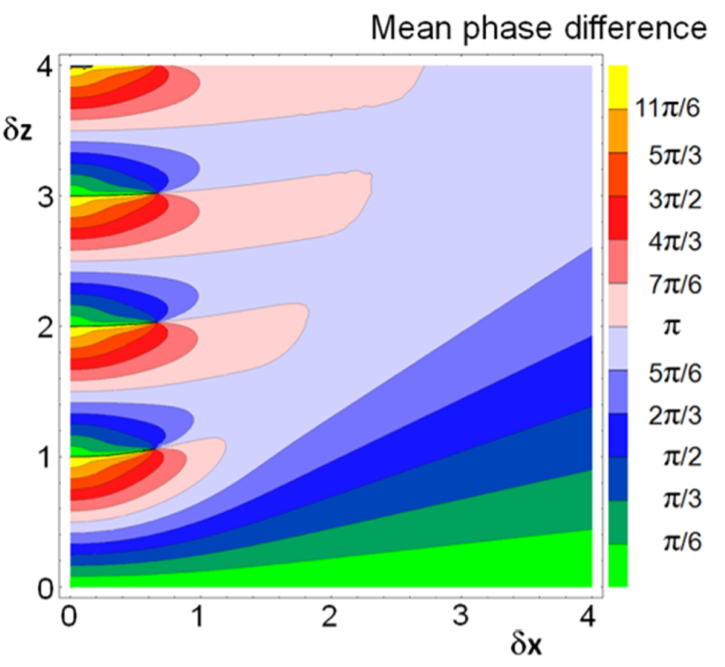
\includegraphics[width=0.8\textwidth]{DopplerModell}
  \caption{Phasendifferenzen im erweiterten Dopplermodell	\cite{Skript}}
  \label{fig:dopplermodell}
\end{figure}

\subsection{Signalverarbeitung}

Um die Signale aus dem OCT zu verarbeiten, müssen verschiedene Umformungen gemacht werden: Zunächst ein Dechirp, der Verzerrungen ausgleicht, indem er reskaliert. Dann wird über das Spektrum ein Hanning-Fenster gelegt. Dieses schwächt das Rauschen ab, führt aber zu einer Auflösungsverschlechterung. Schließlich wird mit Fast Fourier Transformation das Tiefenprofil erstellt. Die Intensitätsdarstellung wird dabei in die logarithmische Skala überführt und als 8\,bit Grauwert ausgegeben.

\section{Durchführung}

Der Versuch wird mit einem FD OCT-Gerät durchgeführt. Dabei wird die Methode der SD OCT angewandt. Die verwendete Zentralwellenlänge $\lambda_0$ beträgt $845\,nm$ bei einer Bandbreite von $\Delta \lambda = 35\,nm$. Das Auslesen erfolgt mit einer Geschwindigkeit von $11888,2\,Hz$.

\subsection{Time Domain OCT}

Zunächst soll TD OCT durchgeführt werden. Da das Gerät selbst auf FD OCT beruht, muss die TD OCT simuliert werden. Dafür wird auf einem Lautsprecher ein Spiegel angebracht. Somit tauschen der Referenzarm und der Probenarm ihre Funktion. Um die Messung durchzuführen, muss zunächst der Spiegel fokussiert werden. Dann wird der Lautsprecher bei einer Frequenz von $20\,Hz$ zum Schwingen gebracht. Die Aufnahme erfolgt mit dem Programm TD\_OCT.vi. Die Messdaten werden gespeichert.

Um die Geschwindigkeit des Lautsprechers zu bestimmen, muss danach noch mit FD OCT die Amplitude der Schwingung gemessen werden. Dafür wird das Programm \\ OCT\_MAXIMUS\_Doppler.vi verwendet und die aufgenommenen Messdaten wieder gespeichert. 

\subsection{Frequency Domain OCT}

Hier soll zunächst die axiale Auflösung des Geräts untersucht werden. Dafür wird eine aufgeraute, $5\,mm$ dicke Glasplatte in den Strahlengang gehalten und fokussiert, sodass der Oberflächenreflex gut zu sehen ist. Die Daten werden gespeichert.

Als nächstes wird eine medizinische Messung durchgeführt. Dafür werden zwei Finger in den Strahlengang gehalten und fokussiert: Ein eingecremter Finger und ein uneingecremter. Nach der Messung an jeweils drei Stellen der Finger werden beide für 10 Minuten in ein Wasserbad gehalten. Dann wird an den selben Stellen wieder ein Bild aufgenommen. Dies wird nach nochmals 10 Minuten im Wasserbad wiederholt.

\subsection{Doppler FD OCT}

Als letztes soll in einer runden Glaskapillare mit einem Innendurchmesser von etwa $300\, \mu m$ die Fließgeschwindigkeit quantitativ bestimmt werden. Dafür wird eine Lösung aus $2\,ml$ Intralipid20 und $48\,ml$ destilliertem Wasser hergestellt. Dann wird der tatsächliche Innendurchmesser an der untersuchten Stelle gemessen, indem dort ein Bild der leeren Kapillare nach der Fokussierung aufgenommen wird. Dann wird zur Bestimmung des Brechungsindex der Kapillare ein Bild der mit der Lösung durchsetzten Kapillare gemacht. 

Zur Bestimmung der Fließgeschwindigkeit muss zunächst der korrekte Dopplerwinkel eingestellt werden. Danach wird ein Volumenstrom eingestellt, der zu einer maximalen Fließgeschwindigkeit unterhalb der Schwelle zum erweiterten Dopllermodell führt. Schließlich werden mit dem Programm OCT\_MAXIMUS\_Doppler.vi die Geschwindigkeitsprofile aufgenommen und gespeichert. 

\section{Analyse}

Längenmessungen während der Analyse: In den aufgenommenen Bildern können mit verschiedenen Bearbeitungsprogrammen Abstände in der "`Einheit"' Pixel gemessen werden. Ein Pixel in y-Richtung ist dabei $5\, \mu m$ groß. Hierrüber kann also die tatsächliche Länge ausgerechnet werden.

\subsection{Time Domain OCT}

\begin{figure}[ht]
	\centering
	  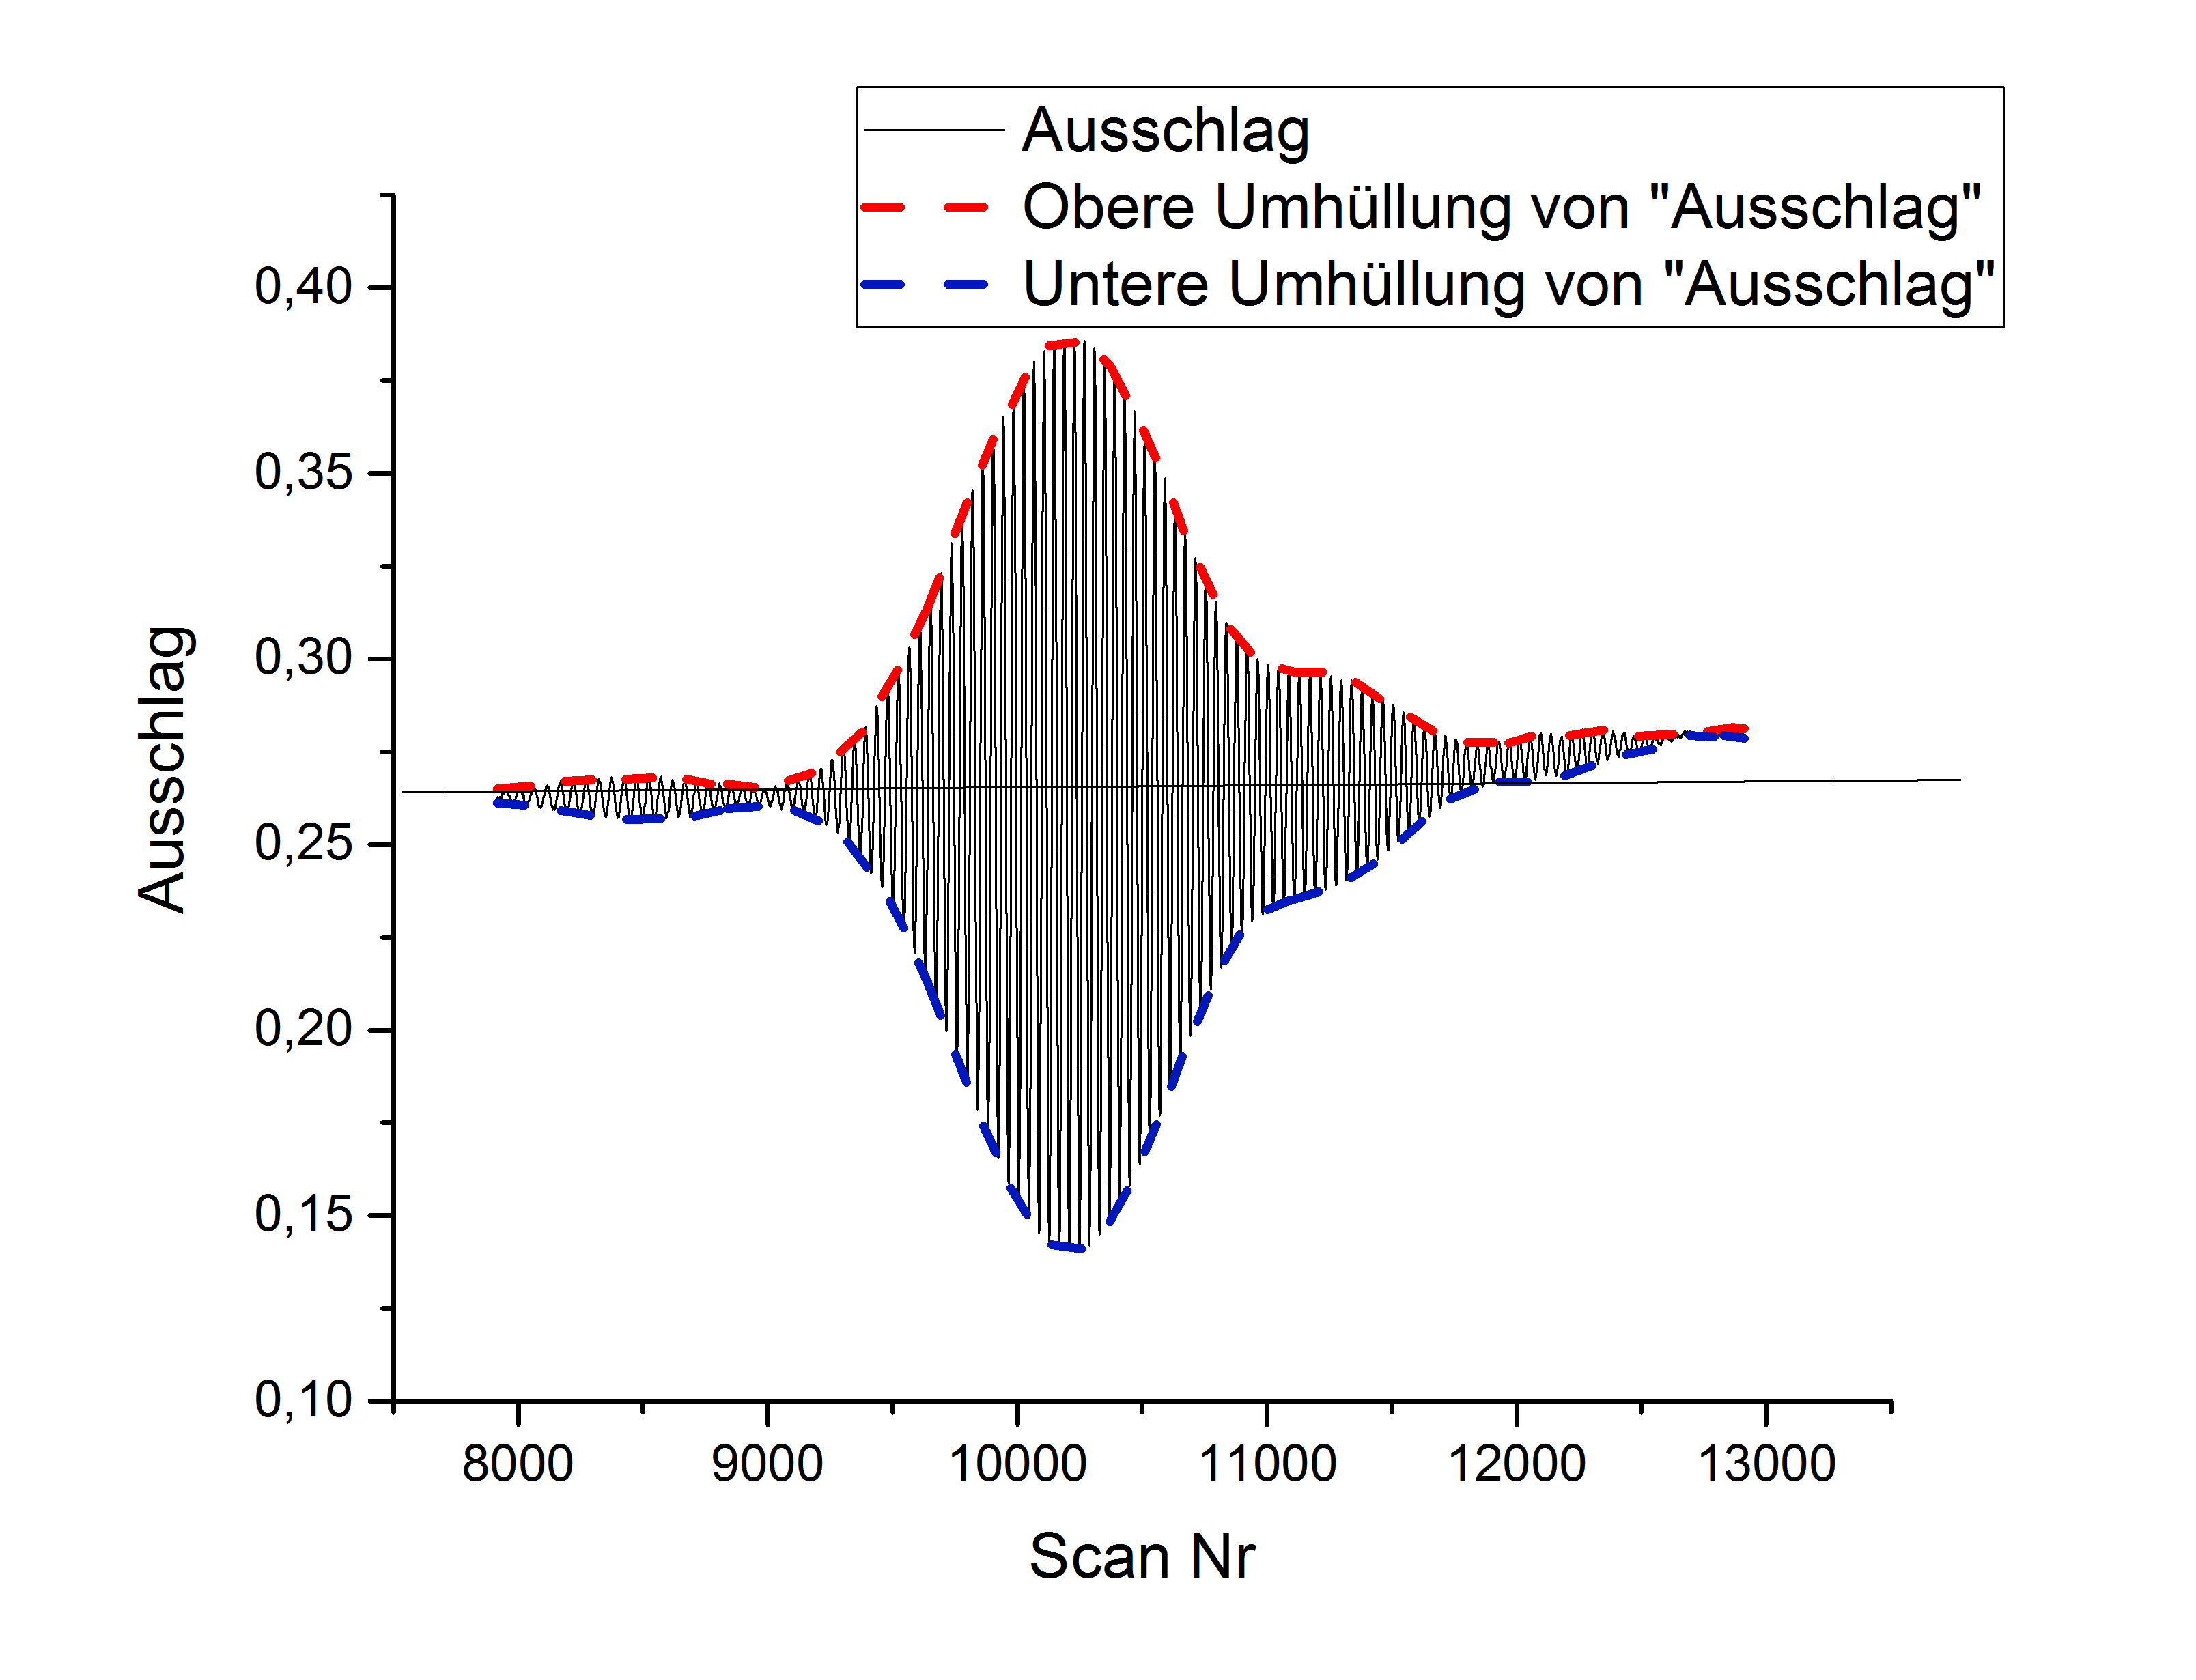
\includegraphics[width=\textwidth]{TD_OCT_DATA_Einhullende}
	\caption{Mit TD OCT gemessene Ausschlagsfunktion des Lautsprechers}
	\label{fig:Funktion}
\end{figure}
\begin{figure}[ht]
  \centering
	  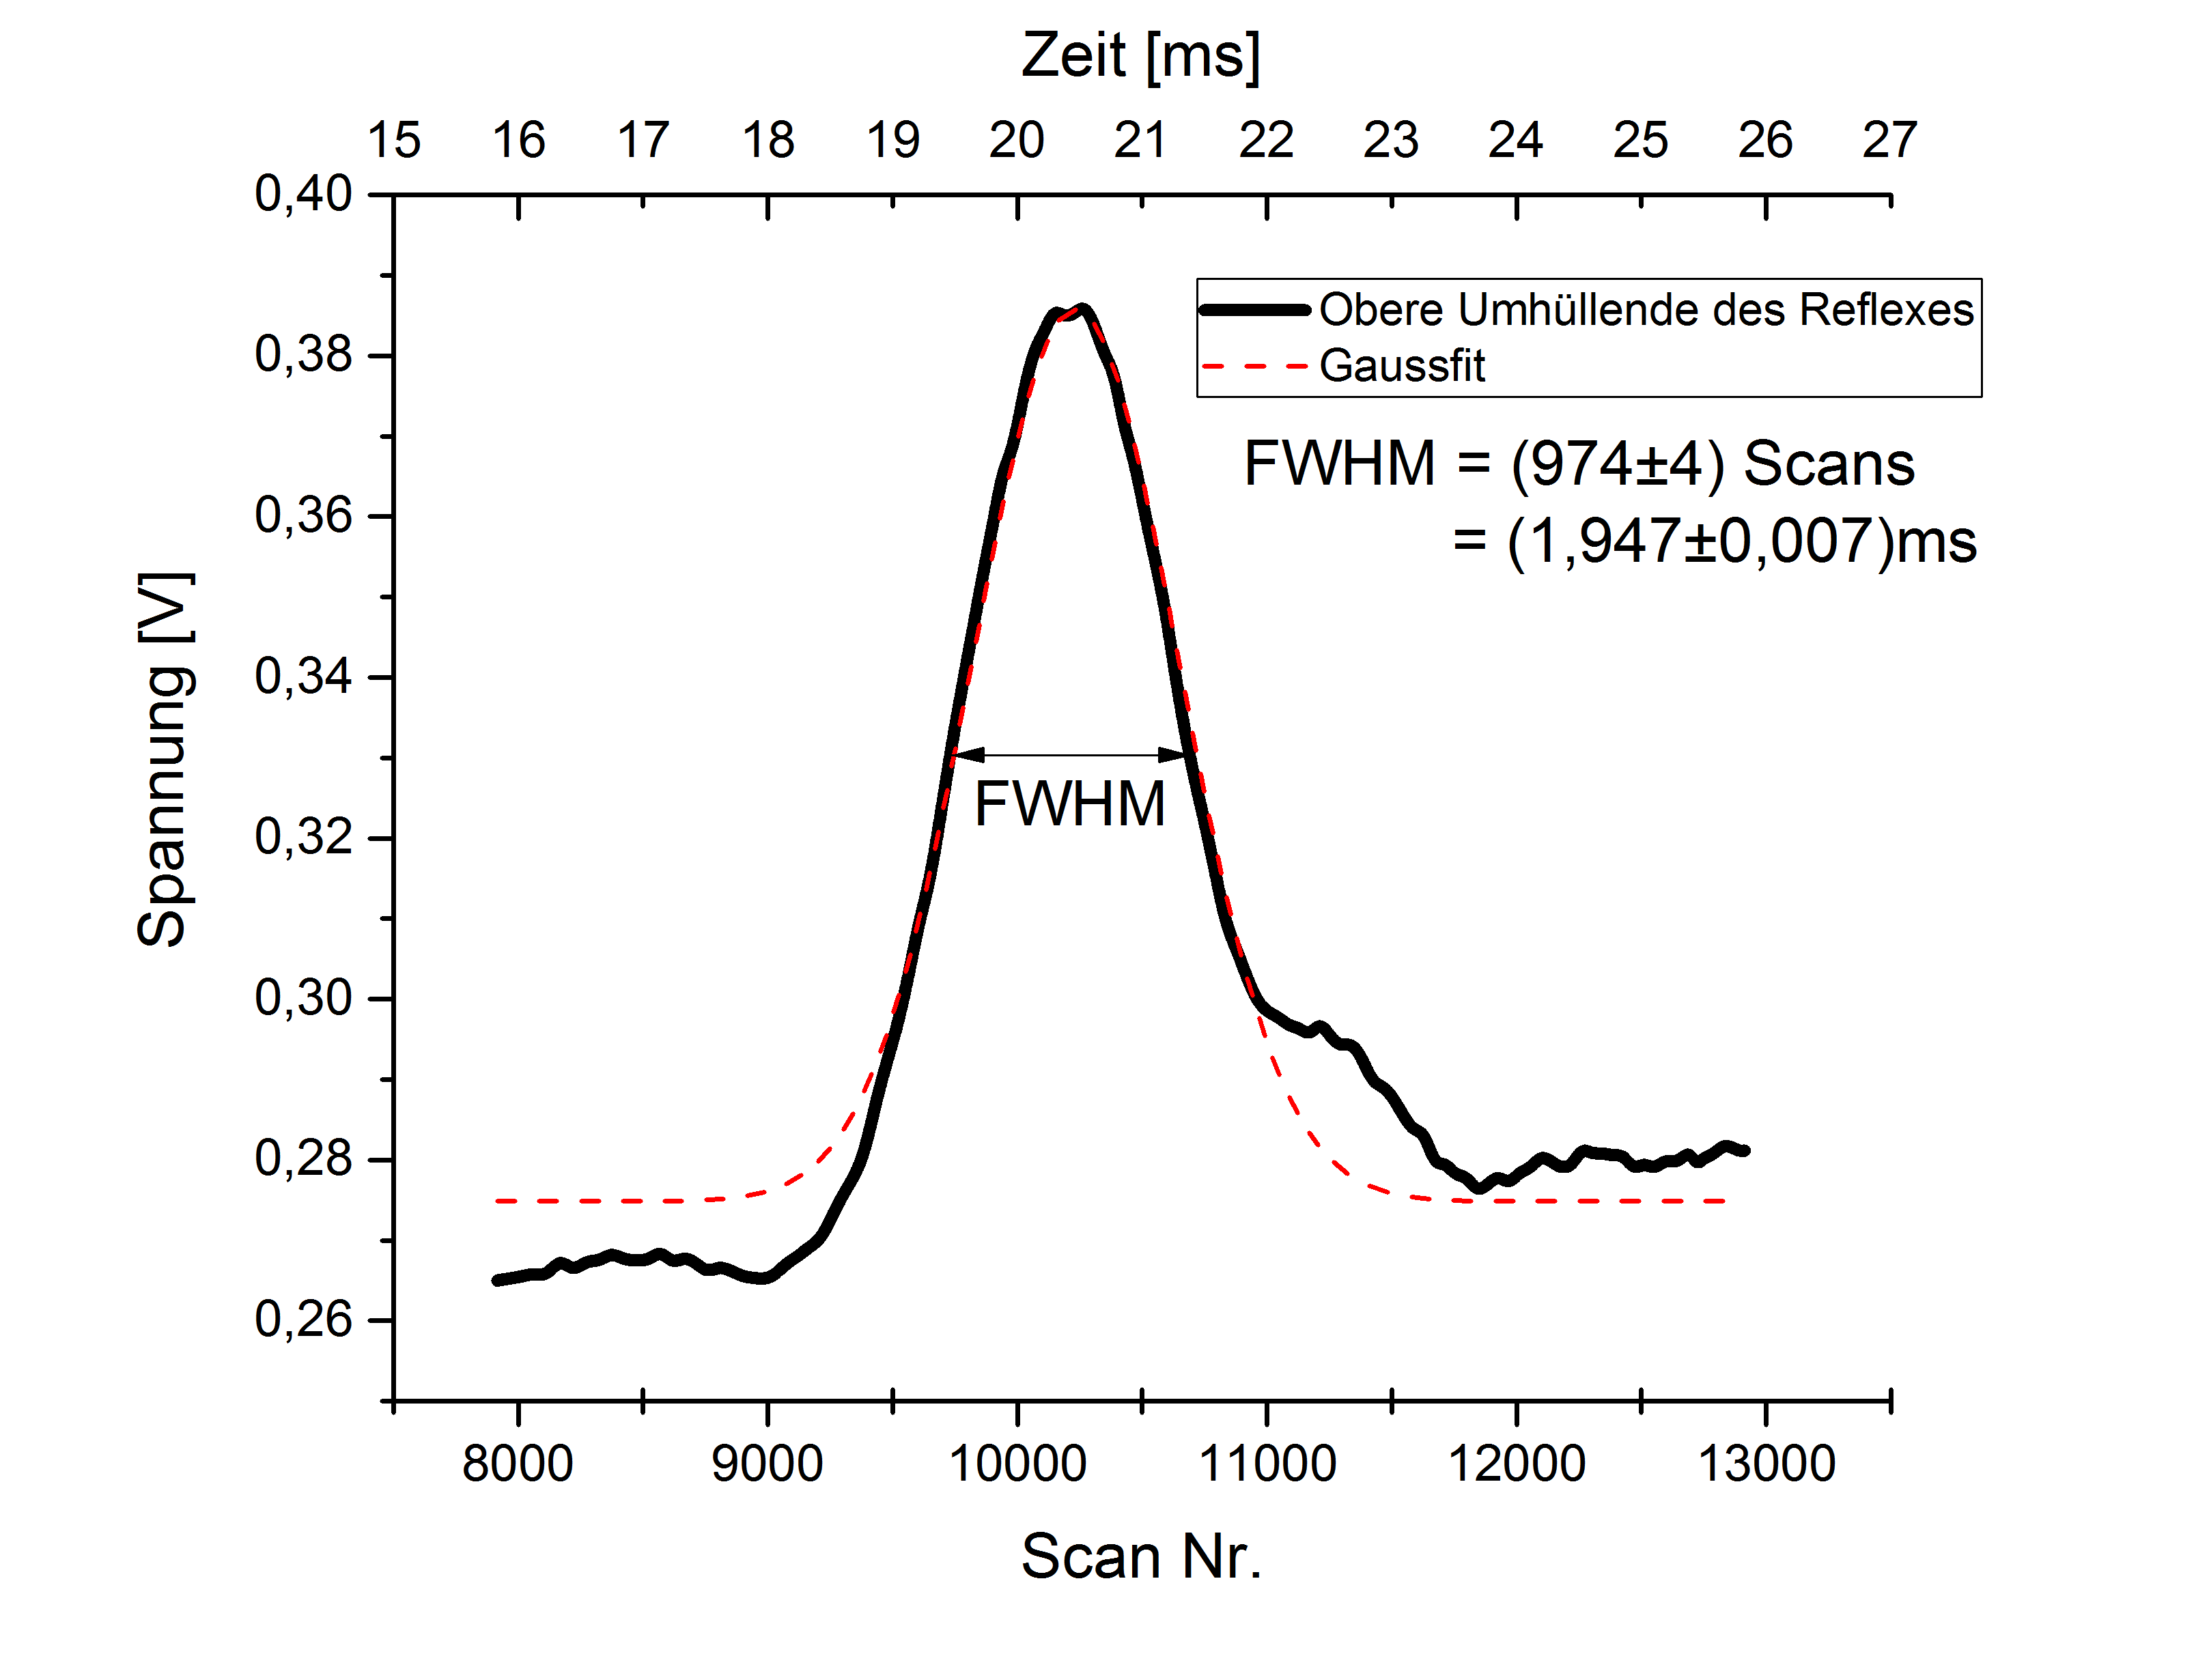
\includegraphics[width=\textwidth]{TD_OCT_FINAL}
  \caption{Berechnete Einhüllende der Funktion}
	\label{fig:hull}
\end{figure}

Die Frequenzfunktion wird mit der simulierten TD OCT aufgenommen. Die Einhüllende dieser Funktion (siehe Bild \ref{fig:Funktion})erinnert an zwei gegeneinander gelegte Gausskurven. Sowohl an die Unter- als auch an die Oberseite kann daher ein Gauss-Fit angelegt werden, wie in Bild \ref{fig:hull} zu sehen ist. Aus diesem Fit lässt sich die Schwingungsdauer und die daraus abgeleitete Frequenz bestimmen. Als Fehler dient die über 4 Werte ermittelte Standardabweichung.
\begin{align*}
T_{Schwingung} = (0.0253 \pm 0.0007) s \\
f_{Schwingung} = (19.802 \pm 0.020) \frac{1}{s}
\end{align*}

\begin{figure}[hb] 
  \centering
    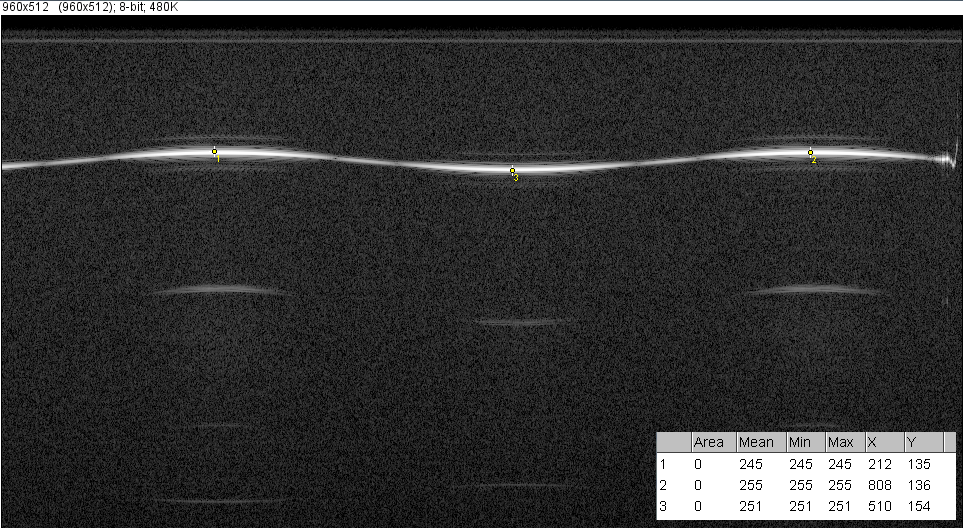
\includegraphics[width=0.7\textwidth]{Amplitude_Beispiel}
  \caption{Auswertung der aufgenommenen Schwingungsamplitude des Lautsprechers}
  \label{fig:amplitude}
\end{figure}

Die Schwingungsamplitude wird mit FD OCT aufgenommen. Das entstandene Bild kann in Bild \ref{fig:amplitude} gesehen werden. Auch hier wird als Fehler die Standardabweichung über 4 Werte gewählt.
\begin{align*}
l_{Amplitude} = (49 \pm 4) \mu m
\end{align*}

Die experimentelle Auflösung wird aus der Geschwindigkeit des Lautsprechers im Nulldurchgang bestimmt. Dafür muss die Halbwertsbreite der Einhüllenden in Hz bestimmt werden. Hierfür wird verwendet, dass die Samplerate 500\,kHz betrug:
\begin{align}
FWHM_{Scans;Hz} = \frac{FWHM_{Scans;Samples}}{500 kHz}
\end{align}
\begin{align*}
FWHM_{Scans;Hz} = (1.948 \pm 0.008) mHz
\end{align*}
\begin{align}
l_{c, TD OCT; exp.} = v_{max; Lautsprecher} FWHM_{Scans;Hz}
\end{align}

Die Geschwindigkeit wird mit der Frequenz des Lautsprechers und der Amplitude über folgende Formel berechnet:
\begin{align}
v_{max; Lautsprecher} = l_{Amplitude} 2 \pi f_{Schwingung} 
\end{align}
\begin{align}
\Delta v_{max; Lautsprecher} = \sqrt{(2 \pi f_{Schwingung} \Delta l_{Amplitude})^2 + (2 \pi \Delta f_{Schwingung} l_{Amplitude})^2}
\end{align}

Der Fehler berechnet sich über die Gauss'sche Fehlerfortpflanzung. Es folgt:
\begin{align*}
v_{Lautsprecher} = (6.1 \pm 0.5) \frac{mm}{s}
\end{align*}
 
Damit ergibt sich der folgende Wert:
\begin{align*}
l_{c, TD OCT; exp.} = (11.9 \pm 1.0) \mu m
\end{align*}

Die theoretische Auflösung der TD OCT wird mit der Formel 2 berechnet. 
\begin{align*}
l_{c, TD OCT; th.} = 9.0022 \mu m
\end{align*}

Das Verhältnis der beiden Auflösungen ist damit folgendes:
\begin{align*}
\frac{l_{c, TD OCT; exp.}}{l_{c, TD OCT; th.}} = 1.32 \pm 0.11
\end{align*}

Die experimentelle erreichte Auflösung ist also etwas schlechter als die theoretisch erreichbare Auflösung. Da ein experimenteller Aufbau aber nie an das Ideal heranreichen wird, ist diese Abweichung durchaus zu erwarten.

\subsection{Frequency Domain OCT}

\begin{figure}[ht]
	\centering
	  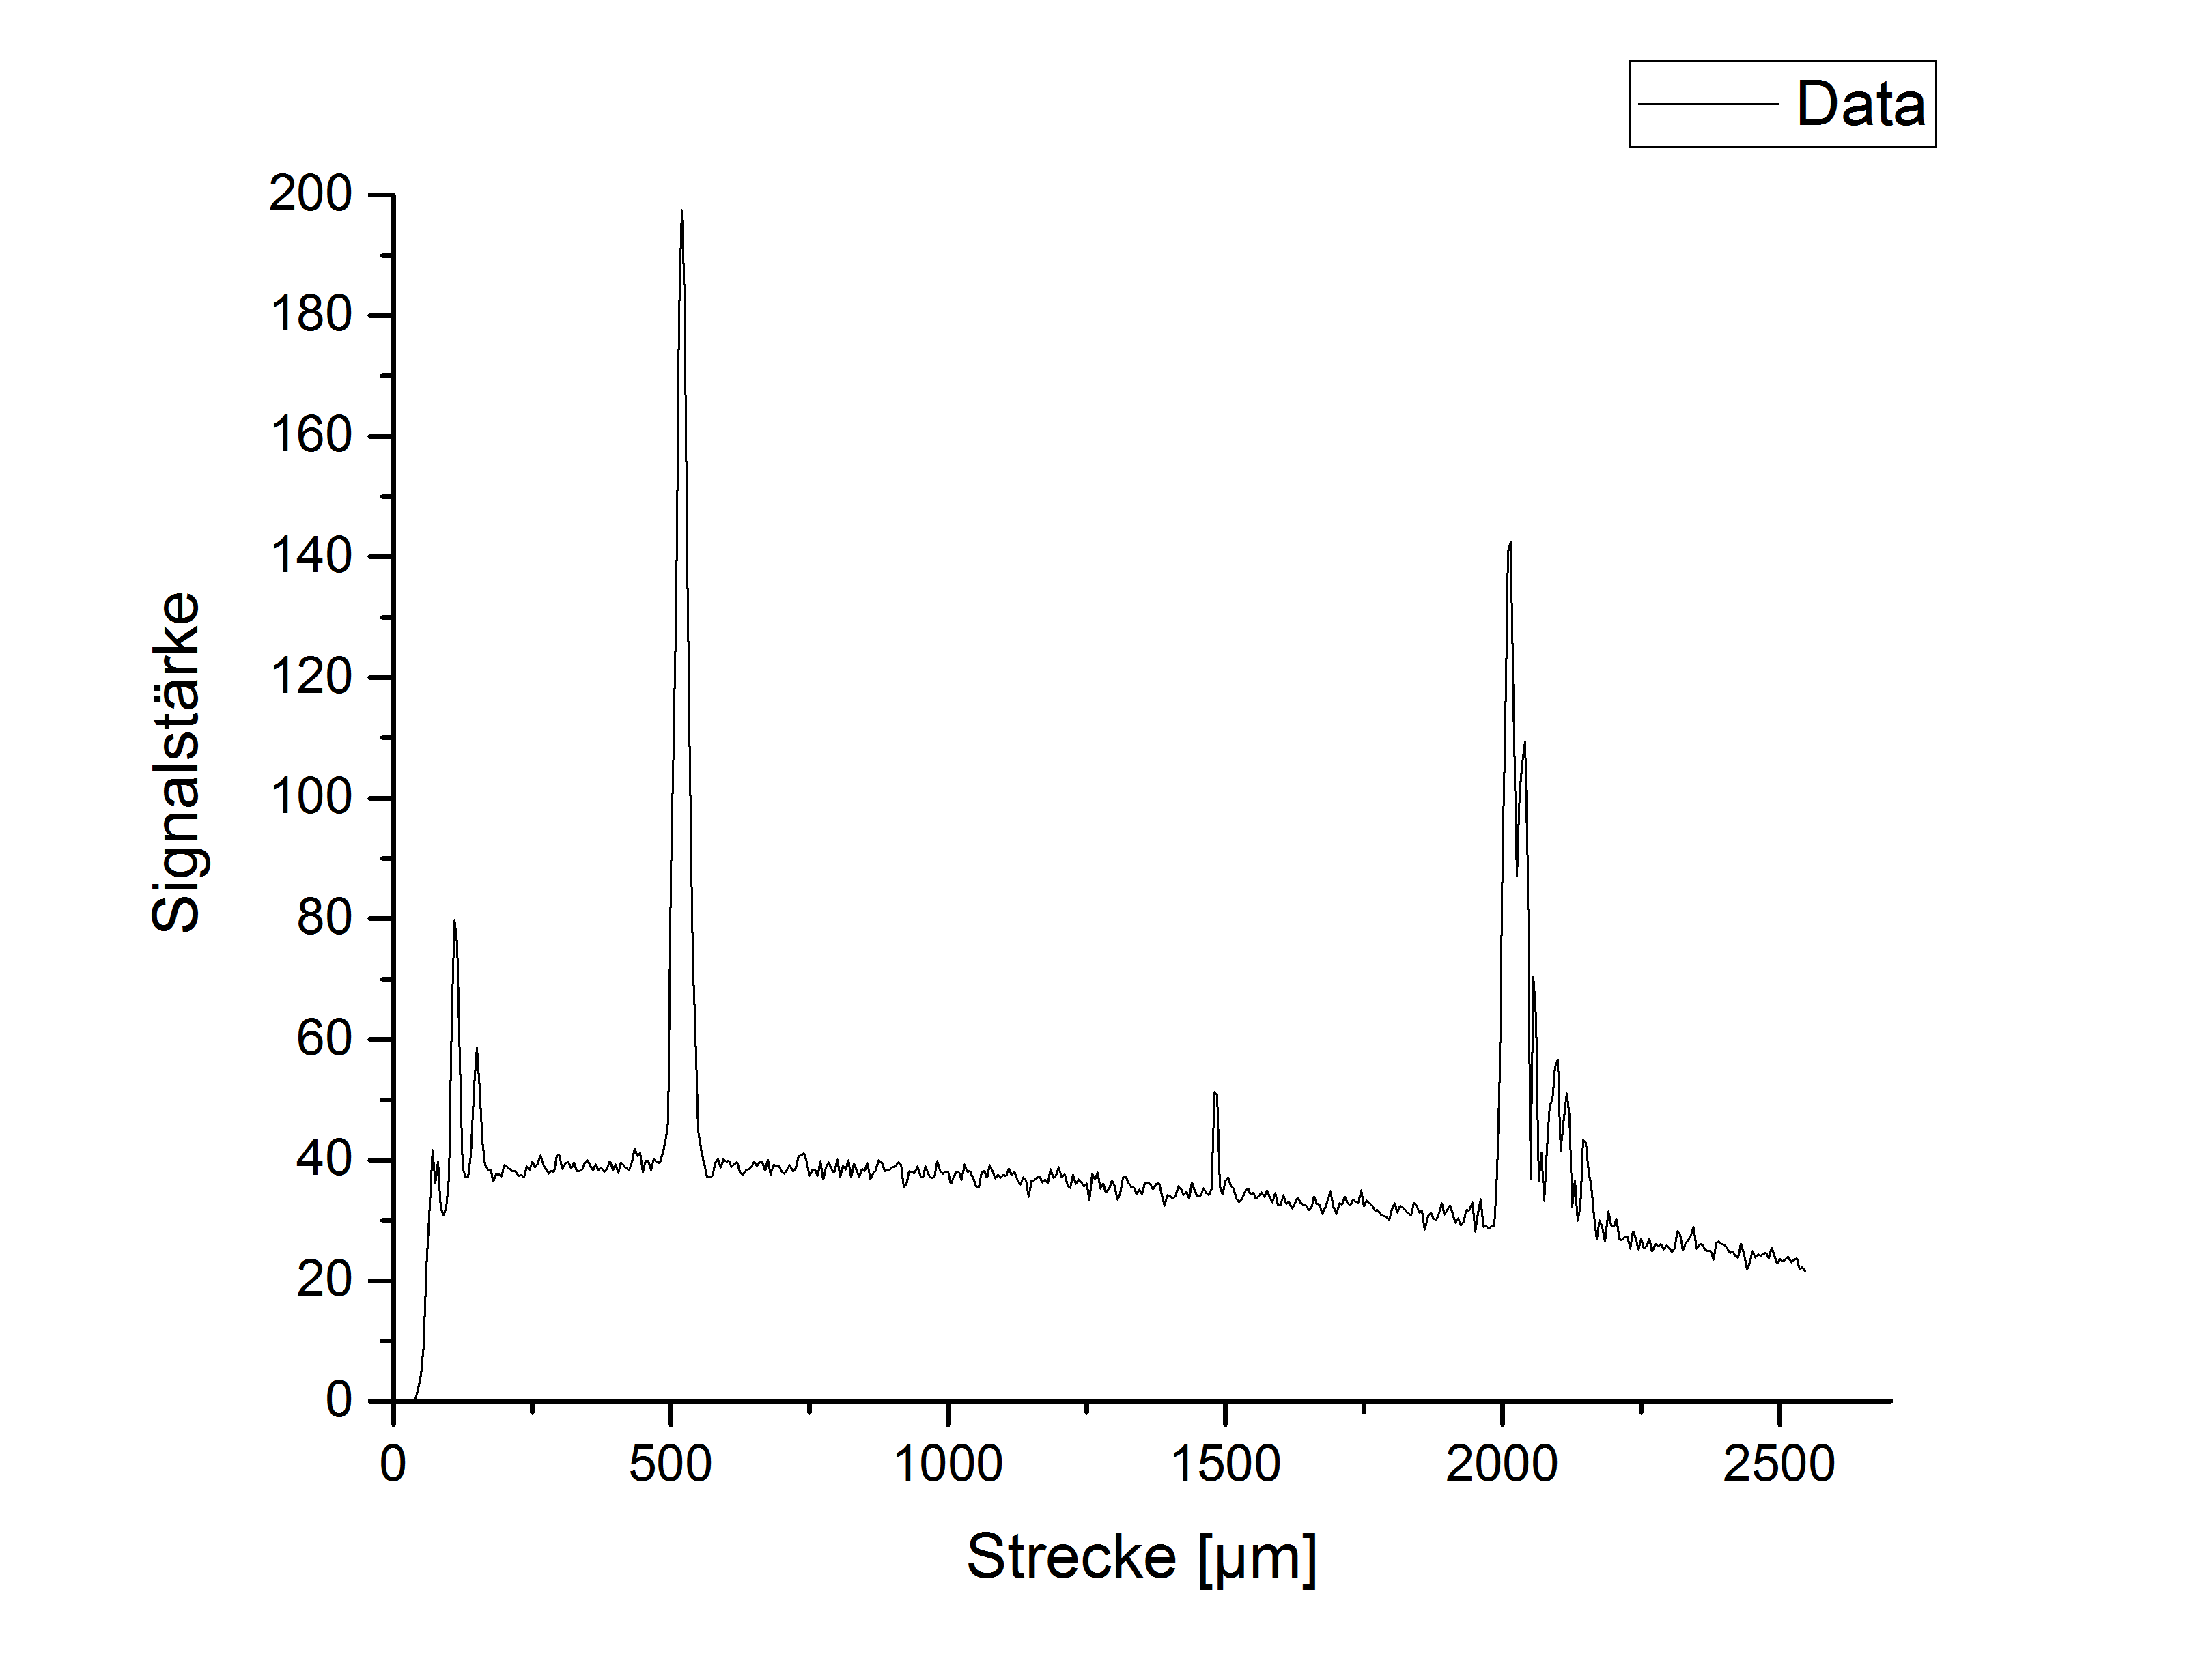
\includegraphics[width=\textwidth]{Glasplattenreflex}
  \caption{Gesamtes Rückstreuspektrum}
	\label{fig:Spektrum}
\end{figure}
\begin{figure}[ht]
  \centering
	  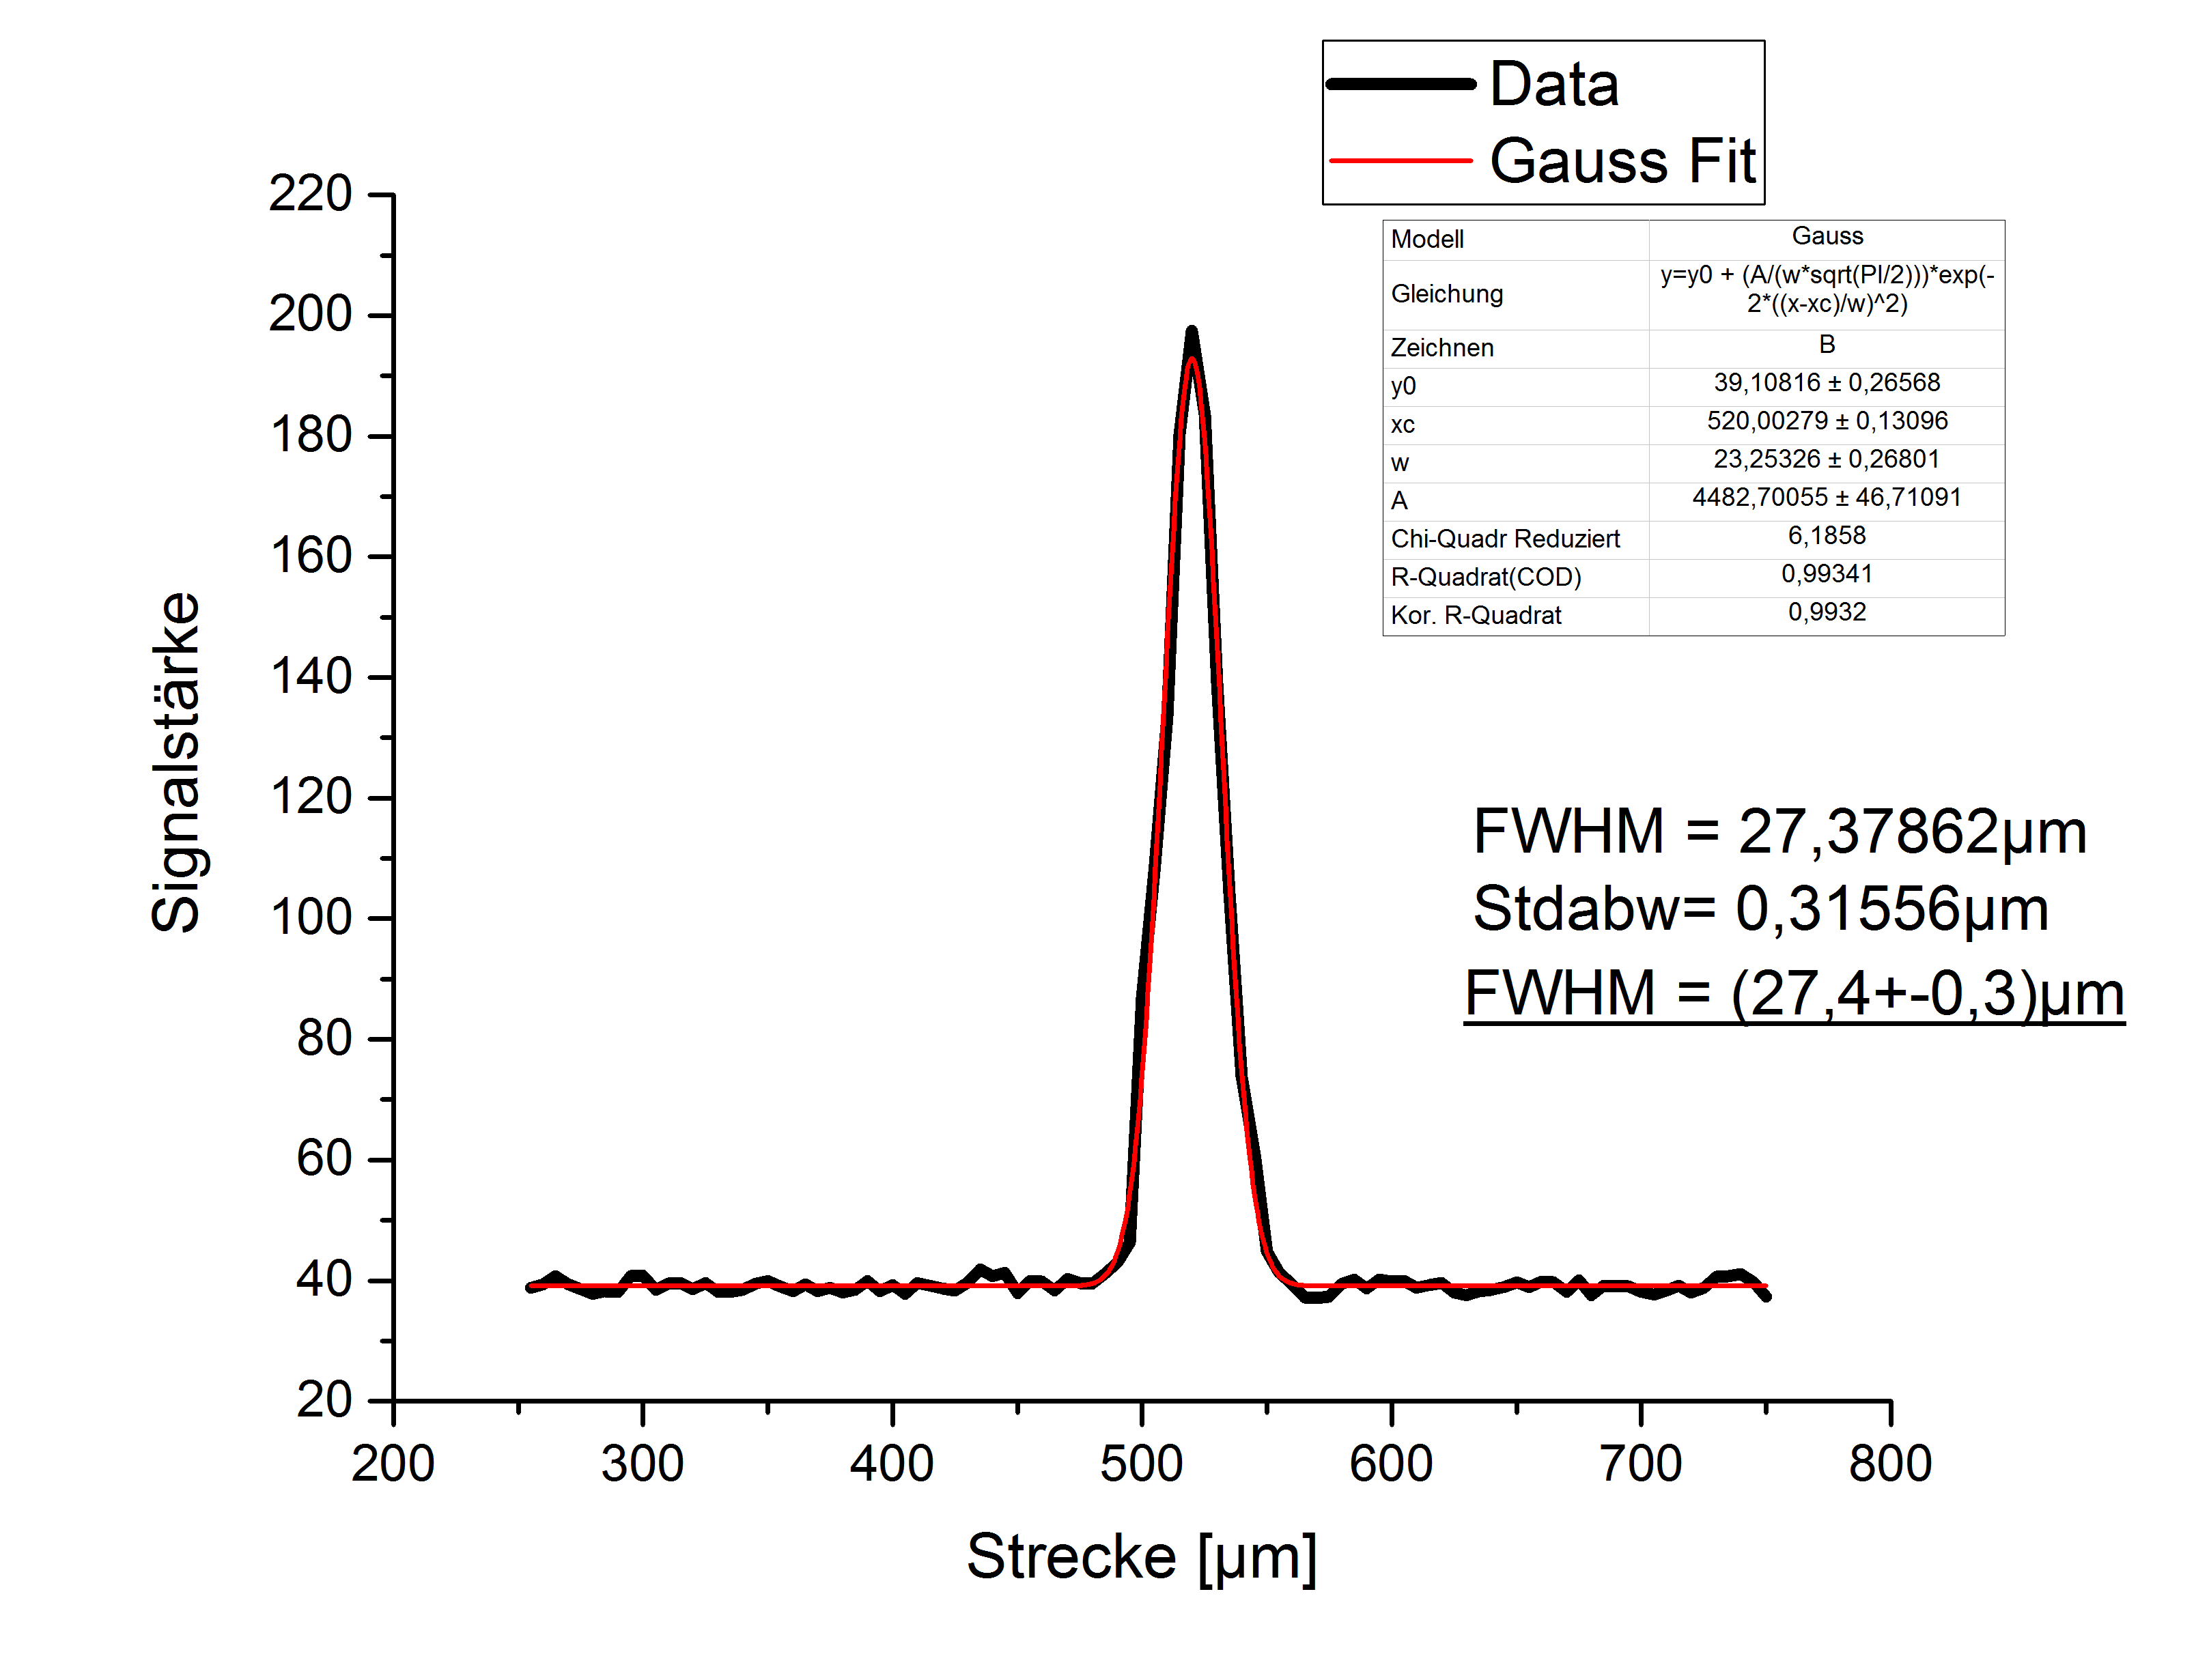
\includegraphics[width=\textwidth]{Ergebnis}
	\caption{Details des Rückstreupeaks}
	\label{fig:peak}
\end{figure}

Zur Bestimmung der experimentellen axialen Auflösung der FD OCT wird das Rückstreuspektrum einer Glasplatte untersucht. Dieses Spektrum zeigt einen Peak, dessen Halbwertsbreite der Halbwertsbreite FWHM\textsubscript{z} entspricht und damit mit der axialen Auflösung l korrespondiert. Das Rückstreuspektrum kann in Bild \ref{fig:Spektrum}, der Peak in Bild \ref{fig:peak} gesehen werden. Da unsere Glasplatte allerings nicht angeraut war und sich daher keine Gitterstreuung mit einem scharfen 0. Maximum ergab, ist die gemessene Halbwertsbreite vermutlich größer als die tatsächlich mit dem Versuchsaufbau Mögliche.
\begin{align*}
l_{FD OCT; exp.} = (27.4 \pm 0.3) \mu m
\end{align*}

Die theoretische Auflösung der FD OCT lässt sich mithilfe der Formel 3 bestimmen. Dabei stellt die spektrale Bandbreite $\Delta \lambda$ des Lasers FWHM\textsubscript{$\lambda$} da. Da der Brechungsindex des Glases nicht gegeben ist, wird der normale Brechungsindex für Fensterglas 1.5 angenommen. 
\begin{align*}
l_{FD OCT; th.} = 6.00 \mu m
\end{align*}

Damit ergibt sich für das Verhältnis der beiden Auflösungen folgendes:
\begin{align*}
\frac{l_{FD OCT; exp.}}{l_{FD OCT; th.}} = 4.57 \pm 0.05
\end{align*}

Die experimentelle Auflösung ist also um ein Vielfaches schlechter als die theoretisch mögliche. Dies deckt sich sehr gut mit der Vermutung der Peakaufbreitung durch die nicht-angeraute Glasplatte. 

Im folgenden wird die Auswirkung von Wasser auf die Haut der Fingerspitzen untersucht. Dabei zeigen die Bilder \ref{fig:uncreme} das Verhalten eines uneingecremten und die Bilder \ref{fig:creme} das Verhalten eines eingecremten Fingers. 

\begin{figure}[ht]
	\centering
	\begin{subfigure}[b]{0.3\textwidth}
	   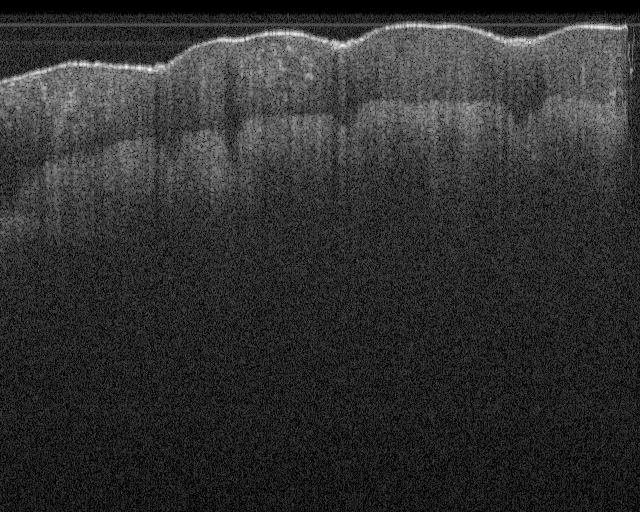
\includegraphics[width=\textwidth]{finger_uncreme_1}
		 \caption{Trocken}
	\end{subfigure}
	\begin{subfigure}[b]{0.3\textwidth}
	   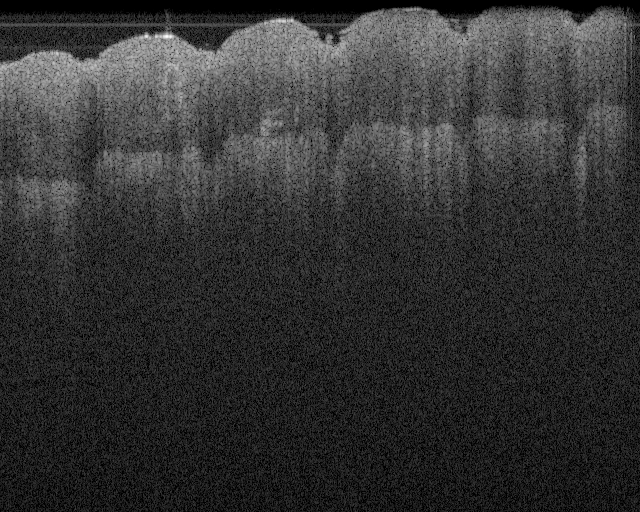
\includegraphics[width=\textwidth]{finger_uncreme_2}
		 \caption{10 Minuten Wasserbad}
	\end{subfigure}
	\begin{subfigure}[b]{0.3\textwidth}
	   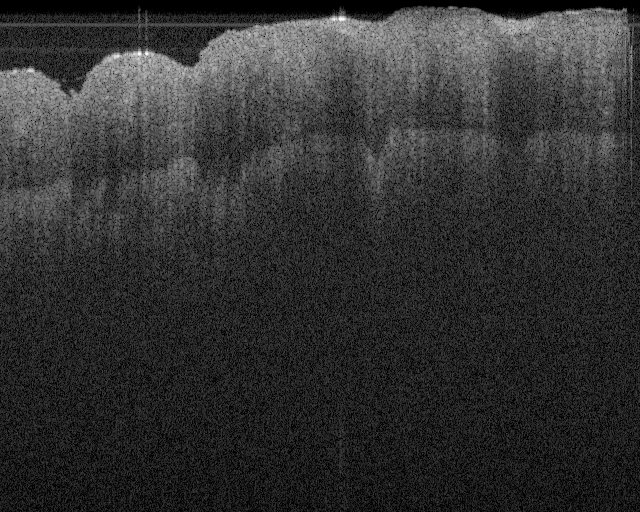
\includegraphics[width=\textwidth]{finger_uncreme_3}
		 \caption{20 Minuten Wasserbad}
	\end{subfigure}
  \caption{Uneingecremte Fingerspitze}
	\label{fig:uncreme}
\end{figure}

\begin{figure}[ht]
	\centering
	\begin{subfigure}[b]{0.3\textwidth}
	   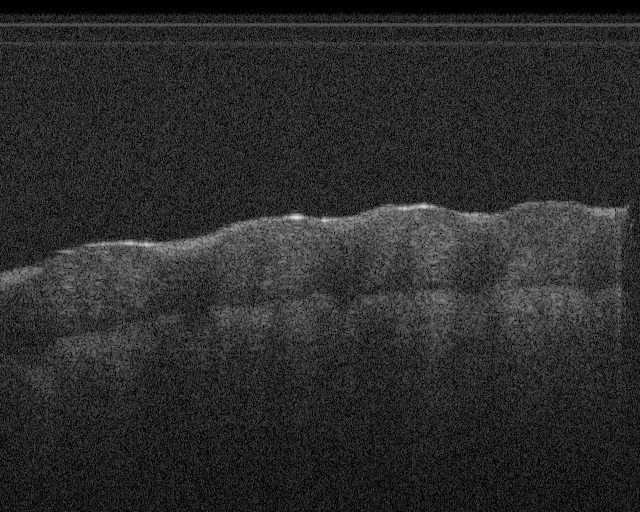
\includegraphics[width=\textwidth]{finger_creme_1}
		 \caption{Trocken}
	\end{subfigure}
	\begin{subfigure}[b]{0.3\textwidth}
	   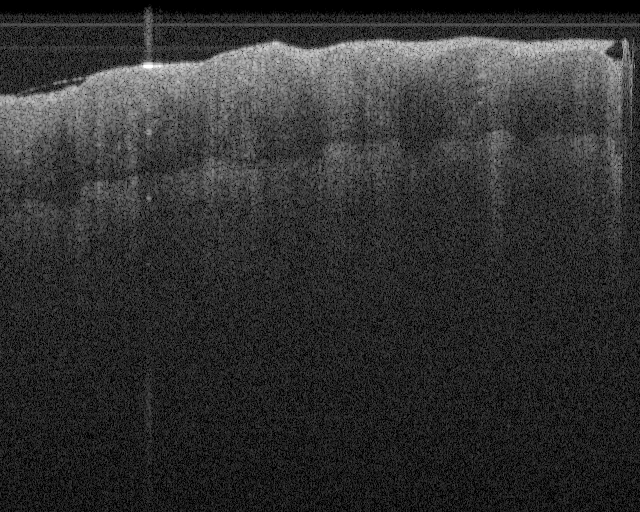
\includegraphics[width=\textwidth]{finger_creme_2}
		 \caption{10 Minuten Wasserbad}
	\end{subfigure}
	\begin{subfigure}[b]{0.3\textwidth}
	   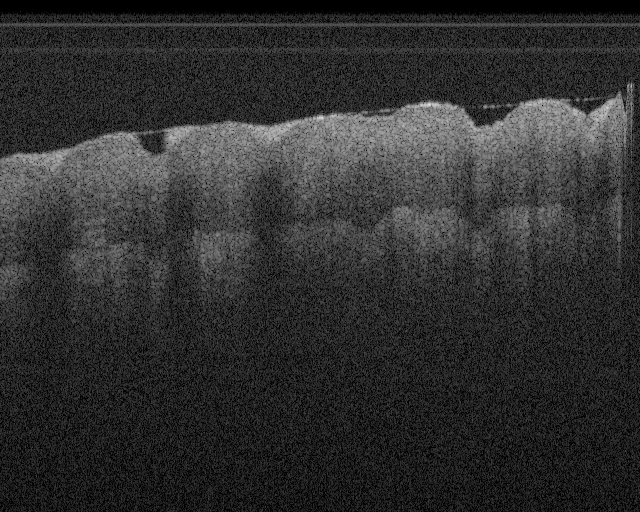
\includegraphics[width=\textwidth]{finger_creme_3}
		 \caption{20 Minuten Wasserbad}
	\end{subfigure}
  \caption{Eingecremte Fingerspitze}
	\label{fig:creme}
\end{figure}

Die Bilder zeigen die oberste Hautschicht (Epidermis) und den Beginn der zweiten Schicht (Dermis). Die eingecremten Finger zeigen zuätzlich eine weiß erscheinende Ablagerung auf der Epidermis, welche vermutlich die Creme darstellt. Grundsätzlich lässt sich erkennen, dass die Einwirkung von Wasser zu einer Vergrößerung der Epidermis führt. Die genauen Werte wurden an den dargestellten Bildern mittels Mittelung von Messungen an 4 Stellen ermittelt und können in Tabelle \ref{tab:finger} eingesehen werden. Dabei wurde zur Berechnung der Dicke in $mm$ verwendet, dass ein Pixel $5 \mu m$ entspricht und die Epidermis einen Brechungsindex von 1.45 hat \cite{brechung}:
\begin{align}
d_{Epidermis; mm} = \frac{d_{Epidermis; Pixel}5\mu m}{n_{Epidermis}}
\end{align}

\begin{table}[ht]
\centering
\begin{tabular}[h]{p{2cm}|p{2cm}|p{2cm}|p{2cm}|p{2cm}|p{2cm}|p{2cm}}
& \multicolumn{3}{c|}{ohne creme} & \multicolumn{3}{c}{mit creme} \\ \hline
Messung & Messwerte [Pixel] & Mittelung [Pixel] & Mittelung [$mm$] & Messwerte [Pixel] & Mittelung [Pixel] & Mittelung [$mm$]\\ \hline
\multirow{4}{*}{Trocken} & 81 & \multirow{4}{*}{79.75} & \multirow{4}{*}{0.275} & 83 & \multirow{4}{*}{83.75} & \multirow{4}{*}{0.289} \\
& 75 & & & 81 & & \\
& 82 & & & 90 & & \\
& 81 & & & 81 & & \\ \hline
& 120 & \multirow{4}{*}{110.25} & \multirow{4}{*}{0.380} & 102 & \multirow{4}{*}{108.25} & \multirow{4}{*}{0.373} \\
10 Minuten & 114 & & & 117 & & \\
Wasser & 103 & & & 106 & & \\
& 104 & & & 108 & & \\ \hline
& 121 & \multirow{4}{*}{124.25} & \multirow{4}{*}{0.428} & 103 & \multirow{4}{*}{103.75} & \multirow{4}{*}{0.358} \\
20 Minuten & 117 & & & 104 & & \\
Wasser & 131 & & & 111 & & \\
& 128 & & & 97 & & \\ \hline
\end{tabular}
\caption{Dicke der Epidermis vor und nach Wassereinwirkung}
\label{tab:finger}
\end{table}

Es zeigt sich, dass der eingecremte Finger weniger aufquillt als der uneingecremte Finger, die Creme schützt den Finger also vor dem Eindringen von Wasser. Dies wird vermutlich durch den hohen Fettgehalt bedingt - Fett stößt Wasser ab. Die Abschwellung des uneingecremten Fingers nach 20 Minuten hingegen ist vermutlich auf Messfehler zurück zu führen.
Auf eine Fehlerberechnung wird aufgrund der ungenauen Datenaufnahme verzichtet. Der größte Fehler entsteht dadurch, dass sich die beobachteten Stellen nur sehr schlecht wiederfinden lassen und daher die Bilder nur in etwa die selbe Stelle des Fingers zeigen.

\subsection{Doppler FD OCT}

\begin{figure}[ht]
	\centering
	\begin{subfigure}[b]{0.4\textwidth}
		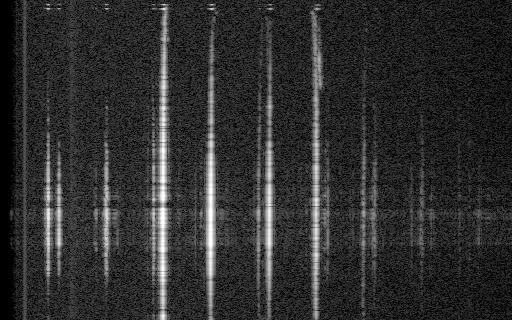
\includegraphics[width=\textwidth]{KapillarLuft}
	  \caption{Ungefülltes Flussphantom}
	  \label{fig:leerkap}
  \end{subfigure}
  \begin{subfigure}[b]{0.4\textwidth}
	  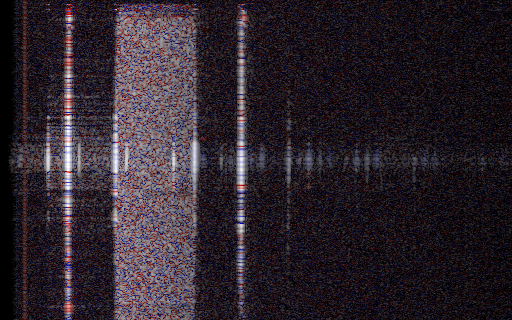
\includegraphics[width=\textwidth]{KapillarEmulsion}
	  \caption{Gefülltes Flussphantom}
	  \label{fig:fuelkap}
  \end{subfigure}
\end{figure}

Als erstes soll überprüft werden, wie groß der Durchmesser des Flussphantoms an der untersuchten Stelle wirklich ist. Dafür wird ein Bild des leeren Phantoms aufgenommen, welches in Bild \ref{fig:leerkap} gesehen werden kann. 
\begin{align*}
d_{Flussphantom} = (290.5 \pm 6.5) \mu m
\end{align*}

Damit ist die untersuchte Stelle etwas schmaler als die ursprünglich angenommenen $300\, \mu m$.

Dann wird der Brechungsindex der Intralipid20-Lösung ermittelt. Dafür wird der Kapillardurchmesser auch im Bild des Flussphantoms gefüllt mit Emulsion (Bild \ref{fig:fuelkap}) in Pixeln gemessen und das Verhältnis der beiden gemessenen Durchmesser berechnet: 
\begin{align}
n_{Intralipid20} = \frac{d_{Intralipid20}}{d_{Luft}}
\end{align}
\begin{align*}
d_{Luft} = (58.1 \pm 1.3) Pixel \\
d_{Intralipid20} = (80.6 \pm 1.3) Pixel \\
n_{Intralipid20} = 1.39 \pm 0.04
\end{align*}

Nun wird das Geschwindigkeitsprofil im Phantom betrachtet. Dabei muss eine Geschwindigkeit eingestellt werden, die eine Verschiebung unterhalb der Grenze $\delta x = 1$ hervorruft. Der dafür notwendige Volumenstrom $\dot V$ kann mit folgender Formel berechnet werden: 
\begin{align}
\dot V = \frac{\pi R^2 \omega_0 f_{Scans} \delta_x}{2 \cos (\theta)}
\end{align}
Wobei R der Radius des Phantoms ist, $f_{Scans}$ die Auslesefrequenz und $\theta$ der Winkel zwischen betrachteter und tatsächlicher Geschwindigkeit der Lösung. Der einzustellende Winkel ergibt sich aus dem Modell in Abbildung \ref{fig:dopplermodell}, es soll ein Winkel gefunden werden, bei dem das unkorrigierte Doppler-Modell noch greift und der gleichzeitig möglichst groß ist, damit der verwendete Volumenstrom größtmöglich ist. Der gefundene Maximalwinkel $\theta_0$ beträgt etwa $2.69^\circ$. Durch den Brechungsindex der Lösung verschiebt sich der beobachtete Winkel jedoch. Der tatsächlich einzustellende Winkel berechnet sich über:
\begin{align}
\theta = \theta_0 n_{Intralipid20}
\end{align}
Und ergibt sich damit zu:
\begin{align*}
\theta = 3.61^\circ
\end{align*}

Daraus folgt, dass folgender Volumenstrom eingestellt werden muss:
\begin{align*}
\dot V = 0.4 \frac{ml}{s}
\end{align*}

In diesem Experiment nahm das Aufnahmegerät jedoch keine Flussgeschwindigkeiten bei diesem Volumenstrom auf, entweder, weil das Programm nicht richtig arbeitete, oder weil die Pumpe nicht richtig funktionierte. Dabei ist eine Fehlfunktion der Pumpe wahrscheinlicher, da keine Pumpgeräusche mehr bei niedrigen Volumenströmen zu hören waren. Wir haben daher mit einem an der Pumpe eingestellten Volumenstrom von $4.4\, ml/s$ gearbeitet, der den niedrigsten Wert darstellte, für den eine Messung möglich war.

\begin{figure}[ht]
	\centering
	  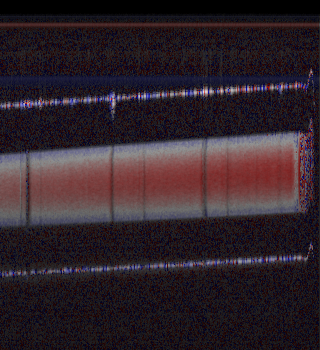
\includegraphics[width=\textwidth]{DopplerFluss}
	\caption{Gemittelte Flussgeschwindigkeit im Kapillar}
	\label{fig:flussbild}
\end{figure}
\begin{figure}[ht]
  \centering
	  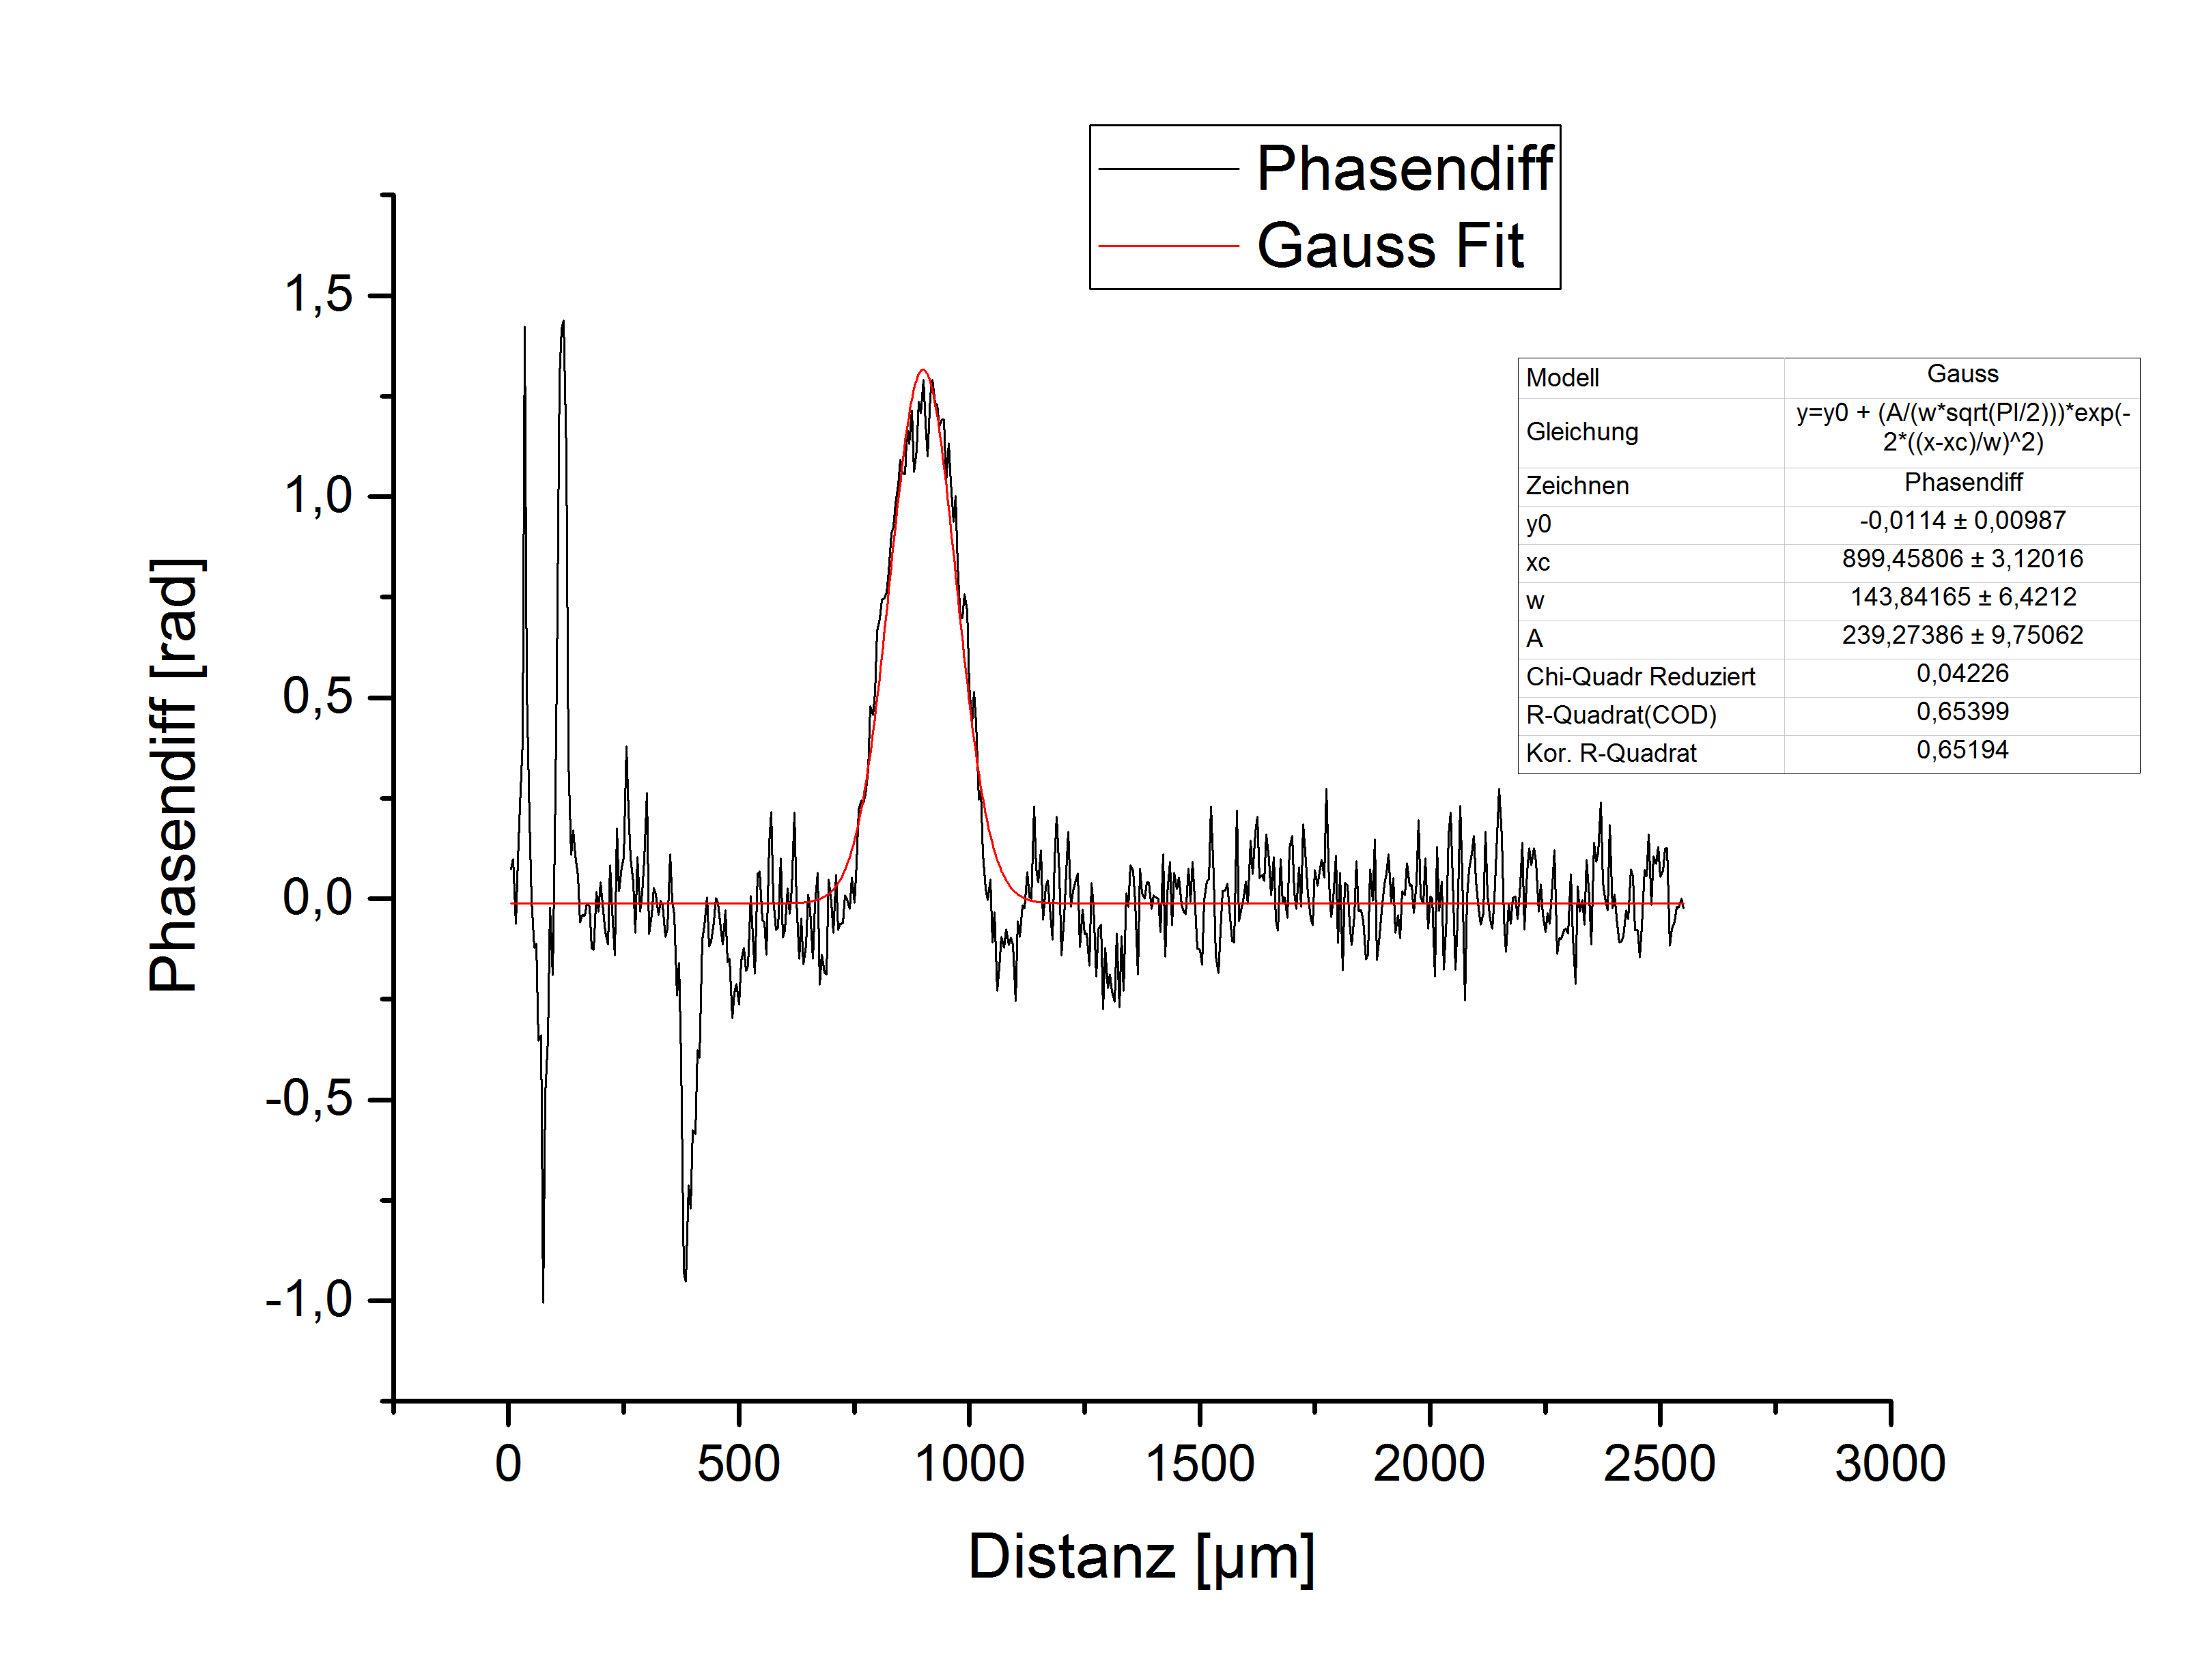
\includegraphics[width=\textwidth]{FlussDiagramm}
	\caption{Gemittelte Flussgeschwindigkeit als Diagramm}
	\label{fig:flussdia}
\end{figure}

Bild \ref{fig:flussbild} zeigt das Bild der Flussgeschwindigkeit im Aufnahmegerät. Die Färbung ist eine Phasenverschiebung, was eine bestehende Flussgeschwindigkeit bedeutet. Das ausgewertete Profil dieser kann in Bild \ref{fig:flussdia} gesehen werden.

\section{Fazit}

\subsection{Time Domain OCT}

\begin{align*}
l_{c, TD OCT; exp.} = (11.9 \pm 1.0) \mu m \\
l_{c, TD OCT; th.} = 9.0022 \mu m \\
\frac{l_{c, TD OCT; exp.}}{l_{c, TD OCT; th.}} = 1.32 \pm 0.11
\end{align*}

Wir konnten feststellen, dass die Auflösung unserer TD OCT, obwohl sie mithilfe eines Spiegels improvisiert wurde, sehr gut an die theoretisch mögliche heranreichte. Die Improvisation als Beispiel für TD OCTzu betrachten ist also durchaus legitim. 
Die Ungenauigkeiten entstehen unter anderem durch die nicht optimale Gausskurve. Das Gerät ließ keine fließende Einstellung für kleine Werte zu, sondern veränderte die Einstellungen nur bei stärkeren Verstellungen. Auch eine nicht optimale Fokussierung und Erschütterungen des nicht-gefederten Versuchstisches führen zu Ungenauigkeiten.

\subsection{Frequency Domain OCT}

\begin{align*}
l_{FD OCT; exp.} = (27.4 \pm 0.3) \mu m \\
l_{FD OCT; th.} = (5.2 \pm 1.0) \mu m \\
\frac{l_{FD OCT; exp.}}{l_{c, FD OCT; th.}} = 5.27 \pm 1.01
\end{align*}







%------------------------

\begin{thebibliography}{9}

\bibitem{bild-tomographie}
  http://www.zwp-online.info/sites/default/files/users/kerstin/kohaerenz3.png
	05.11.2016
	14:30 Uhr

\bibitem{Skript}
  https://tu-dresden.de/med/mf/ksm/ressourcen/dateien/OCT\_Anleitung.pdf?lang=de
	10.11.2016
	14:00 Uhr
	
\bibitem{brechung}
  https://de.wikipedia.org/wiki/Brechungsindex
	14.11.2016
	17:50 Uhr

\end{thebibliography}

\end{document}
